% ============================================================== 4. Results
\section{Results}
\label{sec:results}

\subsection{Reproduction and pre-specified tests}
\label{sec:res-tests}

The re-implemented pipeline met the pre-specified replication tolerance (Gate~1). On FLamby's official
split, model~A reached a pooled BA of 0.615 with FedAvg (three seeds, range 0.579--0.642), 0.604 with
FedProx, 0.623 with SCAFFOLD and 0.750 with pooled training. The FedAvg value is 4.2 points below the
FedAvg baseline of 0.657 reported in the FENDA-FL study \cite{tavakoli2024fendafl}, inside the margin,
and above FLamby's own published FedAvg results (mean 0.534 over five seeds; 0.585 without one failed
seed) \cite{flamby2022}.

Table~\ref{tab:scorecard} lists all pre-specified tests in the order in which they were registered. The
apparent inflation of the primary FedAvg model met Gate~2. H3b was supported for model~A and not for
model~B. The original shrinkage rule (ShrinkFCP) did not meet the RQ4 criterion for either encoder, and
the empirical-Bayes rule (EB-ShrinkFCP) met the same criterion on held-out models for model~A but not for
model~B; because RQ4 and test~5b require success for both encoders, neither is met overall. Transferred
conformal thresholds failed on PAD-UFES-20 as defined in advance. The randomized sibling-exposure experiment (E8) met its pre-specified test. The following subsections
report the results behind each test and the secondary analyses.

\inputtable{Table2_scorecard}

\subsection{Extent of lesion leakage (RQ2)}
\label{sec:res-extent}

Leakage was concentrated in a few clients (Table~\ref{tab:dataset}). In the official FLamby split, 65.9\%
of the test images had a sibling image of the same lesion in training: 92.7\% in client~0, 72.4\% in
client~2, 55.7\% in client~5, 49.3\% in client~3, 3.0\% in client~4 and 0.1\% in client~1. In our
image-level re-splits the corresponding rates were 83.0\%, 68.0\%, 50.2\%, 43.5\%, 2.7\% and 0.2\%
(59.5\% overall; Figure~\ref{fig:leakage}b). Almost all leakage occurred within a client; leakage through
another client affected 0.1\% of the test images, all in clients 1 and 2.

\subsection{Apparent inflation and the effect of sibling exposure (RQ2)}
\label{sec:res-leakage}

Every encoder and training regime looked more accurate on the full image-level test set than on its
new-lesion subset (Figure~\ref{fig:inflation}). For the primary FedAvg model~A, the apparent inflation was
8.1 points (95\% CI 4.7--11.2; seeds 2.4, 8.6 and 13.3 points). It was similar for the frozen encoders,
8.2 points (5.0--11.5) for A-frozen and 8.7 points (5.2--12.6) for model~B, and larger for model~A FedAvg
after 27 rounds (12.4 points, 9.6--15.6) and for model~A pooled training (16.2 points, 12.5--19.4). With
frozen encoders, pooled training showed less inflation than FedAvg (A-frozen 6.1 points, 2.5--9.8;
model~B 7.3 points, 3.6--11.5). The retrained-split difference, which compares the image-level model on
its own test set with the lesion-grouped model on its own test set, pointed the same way in all six
E1 settings (model~A FedAvg 6.9 points, pooled 15.2; A-frozen 7.5 and 6.0; model~B 6.2 and 3.9; three
seeds; the five-seed E2 values in Table~\ref{tab:ba} differ slightly because they include two more
seeds). Apparent melanoma recall was also higher on the full test sets: for model~A FedAvg 0.48--0.54
versus 0.35--0.41 on the new-lesion subsets across the three seeds, and for model~B FedAvg 0.52--0.55
versus 0.37--0.39.

The randomized sibling-exposure experiment (E8) showed that having a sibling image in training raises
accuracy on the same test images (Supplementary~S11). For the pre-specified model~A FedAvg, BA of the fixed
target images was 9.1 points higher when their siblings were in training than when they were not (95\% CI
5.5--12.3; test met), close to the observational apparent inflation of 8.1 points; NLL fell by 0.10 and
the Brier score by 3.6 points. The effect grew with how closely the model fits its training lesions: for
model~A it was 13.3 points (10.1--16.7) for FedPer, 18.6 (15.2--22.2) for pooled and 28.8 (25.3--32.7) for
local-only training, that is 4.2 (0.5--8.1), 9.5 (5.3--13.6) and 19.8 (15.9--24.0) points more than for
FedAvg on the same images. With frozen encoders, the FedAvg effect was similar (A-frozen 8.6 points,
6.2--11.2; model~B 8.0, 5.7--10.5); the two-layer FedPer-style head of model~B showed 21.1 points
(17.5--24.5), 13.0 more than FedAvg (9.3--16.7), whereas the linear pooled and local-only heads of
model~B showed less than FedAvg (4.5 and 6.2 points). Most of the effect occurred in client~0, whose target
lesions have the most siblings (model~A FedAvg 14.2 points, 9.1--19.2; clients 2 and 3: 1.2 and $-1.5$
points with intervals including zero). Melanoma recall of the target images rose by 1.9 (FedAvg) to 16.7
points (local-only). On the non-target test images, which are identical in both arms, BA differed between
the arms by $-2.1$ to $+4.1$ points, which reflects retraining variability; because every target lesion is
exposed in one arm and unexposed in the other, this variability largely cancels in the exposure effect, but
differences between methods of a few points should be read with it in mind. The estimates apply to lesions
with several images.

\begin{figure}[!t]
  \centering
  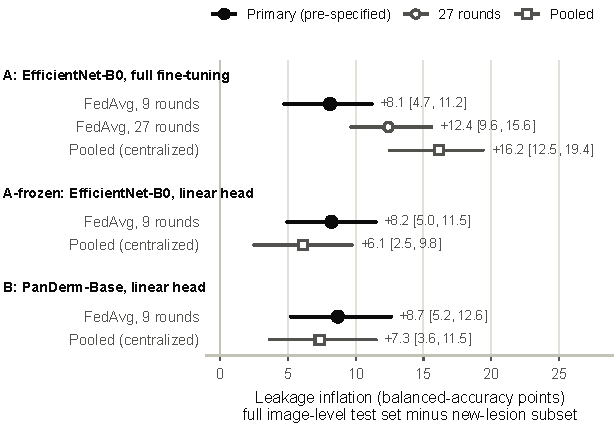
\includegraphics[width=0.62\textwidth]{Fig3_leakage_inflation}
  \caption{Apparent leakage inflation of balanced accuracy (Eq.~\ref{eq:inflation}): BA on the full
  image-level test set minus standardized BA on its new-lesion subset, for the same model (points with
  95\% lesion-bootstrap CI; E1, three seeds). Filled markers: the pre-specified primary FedAvg models.}
  \label{fig:inflation}
\end{figure}

\subsection{Method rankings and accuracy (RQ2, RQ3)}
\label{sec:res-rankings}

Whether leakage changed which method looked best depended on the encoder and the metric
(Figure~\ref{fig:rankings}; Table~\ref{tab:ba}). For model~A and pooled BA, the rankings under the two
split types agreed closely (Kendall's $\tau_b=0.79$, 95\% CI 0.57--0.93), and the agreement of single-seed
rankings across split types (0.66) was close to the seed-to-seed noise floor (0.72). On mean-of-clients
BA, agreement was lower ($\tau_b=0.57$; single-seed 0.24 vs noise floor 0.54), mainly because local-only
training fell from third place on image-level splits to seventh on lesion-grouped splits. For model~B,
rankings on pooled BA were essentially unrelated across split types ($\tau_b=0.05$, $-0.24$ to $0.24$;
single-seed 0.10 vs noise floor 0.74). The FedPer-style two-layer head ranked first on image-level splits
(BA 0.656) and seventh on lesion-grouped splits (0.502). Several of the differences that determine these
ranks are small relative to seed-to-seed variation (Supplementary~S10); for example, model~B FedPer was
2.1 points below FedAvg on lesion-grouped splits (seed range $-5.9$ to $+0.1$). The capacity-matched heads of E9 (Supplementary~S12) indicate that the behaviour of the
FedPer-style head comes from its two-layer architecture rather than from personalization: a FedAvg model
with the same two-layer head showed an apparent inflation of 10.4 points in clients 0, 2 and 3 (FedPer-style
head 10.6, linear FedAvg 6.1) and fell from sixth place on image-level to last place on lesion-grouped
splits (pooled BA 0.606 to 0.466), and the two-layer pooled and local-only heads inflated more than their
linear counterparts (6.4 vs 2.7 and 6.8 vs 4.2 points). With the three two-layer heads added, the agreement
of the model~B rankings across split types remained low ($\tau_b=0.20$, 0.02--0.42; single-seed 0.27 vs
noise floor 0.72).

Pooled BA was lower on lesion-grouped than on image-level test sets for every method and encoder
(Table~\ref{tab:ba}); mean-of-clients BA was not always lower (model~B FedAvg 0.532 vs 0.546). Centralized
pooled training remained best for model~A (pooled BA 0.566). Among the federated methods, FedPer was best
for model~A on pooled BA (0.555, 6.0 points above FedAvg at 0.495; seed range of the difference 1.8 to
10.5), and FedBN on mean-of-clients BA (0.568). For model~B, the federated methods differed by at most
4 points (0.502--0.542), and local-only training reached the highest pooled BA (0.566).

\begin{figure*}[!t]
  \centering
  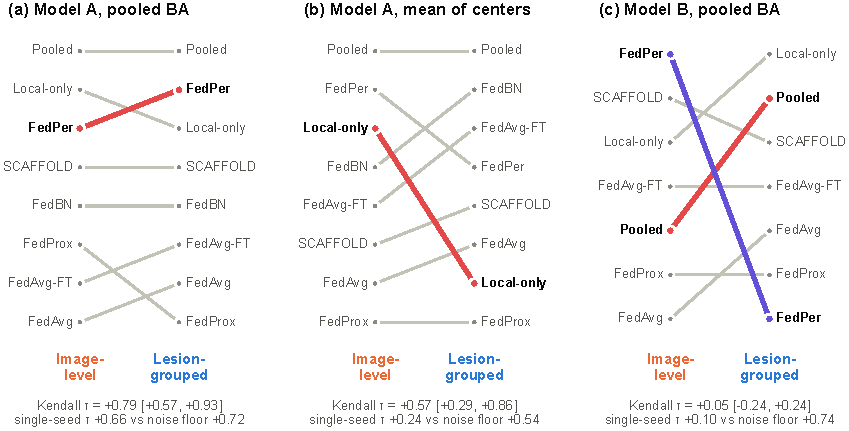
\includegraphics[width=\textwidth]{Fig4_rankings}
  \caption{Method rankings on image-level (left) and lesion-grouped (right) test sets, by mean pooled BA
  over five seeds (top = best). Highlighted methods change rank most. Text below each panel: Kendall's
  $\tau_b$ between the two rankings (95\% CI), and the agreement of single-seed rankings across split types
  compared with the seed-to-seed noise floor.}
  \label{fig:rankings}
\end{figure*}

\inputtable{Table3_balanced_accuracy}

\subsection{Exploratory associations with fitting capacity and feature proximity (RQ3)}
\label{sec:res-mechanism}

In the pre-specified H3b contrast (clients 0, 2 and 3), the local and personalized group of model~A showed
3.2 points more apparent inflation than FedAvg (95\% CI 2.0--4.6; supported), but the difference came
mainly from local-only training (13.7 points) and, to a lesser extent, FedPer (6.7 points); FedBN (4.9) and
FedAvg-FT (4.8) were close to FedAvg (4.3), whereas non-personalized pooled training showed 12.1 points
(Figure~\ref{fig:mechanism}b). For model~B, whose other heads are linear, local-only (4.2) and pooled (2.7)
training showed the least inflation, and the H3b contrast was not supported (0.9 points, $-0.2$ to 2.1).
The FedPer-style two-layer head showed the largest inflation of the model~B methods (10.6 points). These
comparisons span different optimizers, training budgets and head architectures, so they show an
association with how strongly a model fits its training lesions, not a controlled effect of capacity; the
randomized exposure effects of E8 (Section~\ref{sec:res-leakage}) and the capacity-matched heads of E9
(Section~\ref{sec:res-rankings}) order the methods in the same way.

Per-client inflation was larger in clients with more leakage (Figure~\ref{fig:mechanism}a), but this
dose--response is weak evidence. Weighted least-squares slopes ranged from 8.1 points per 100\% leakage
(FedAvg) to 21.5 (local-only) for model~A and from 6.2 to 18.9 for model~B, but client~0 carried most of
the leakage and most of the inflation (10.0 to 22.2 points for model~A), and without client~0 the slopes
ranged from $-2.2$ to 10.0 points for model~A (FedAvg $-1.9$) and from $-1.9$ to 4.1 for model~B
(Supplementary~S3). The slope is also partly built into the measure, because inflation within a class
scales with the leaked share.

An exploratory nearest-neighbor analysis of the frozen embeddings showed why even linear heads can benefit
from leakage (Figure~\ref{fig:mechanism}c; Supplementary Figure~S1). Leaked test images were closer to the
training set than new-lesion images (mean cosine similarity of the centered embeddings to the nearest
training image 0.81 vs 0.75 for A-frozen; 0.85 vs 0.79 for model~B), and for 54\% (A-frozen) and 58\%
(model~B) of the leaked images the nearest training image belonged to the same lesion. A 1-nearest-neighbor
classifier, which fully exploits this proximity, showed 22.7 and 22.4 points of unweighted inflation, and
the linear heads 6.2 and 6.6 points on the same measure. Leaked and new lesions also differ in class and
client composition, so this comparison does not by itself separate proximity from those differences.

\begin{figure*}[!t]
  \centering
  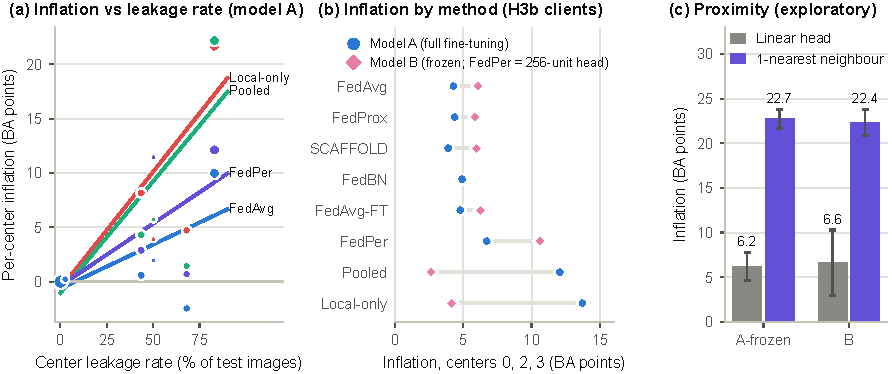
\includegraphics[width=\textwidth]{Fig5_mechanism}
  \caption{Exploratory associations of apparent inflation with leakage rate, method and feature proximity.
  (a) Per-client inflation against the client's leakage rate for four model~A methods, with weighted
  least-squares lines (marker area proportional to the client's new-lesion test images); client~0 carries
  most of the slope (Supplementary~S3). (b) Inflation in clients 0, 2 and 3 (the H3b measure) by method for
  model~A (circles) and model~B (diamonds). (c) Inflation of the frozen-encoder linear heads and of a
  1-nearest-neighbor classifier on the same embeddings (mean $\pm$ SD over seeds; unweighted BA).}
  \label{fig:mechanism}
\end{figure*}

\subsection{Calibration (RQ1, RQ2)}
\label{sec:res-calibration}

Calibration differed more between clients than between methods (Figure~\ref{fig:calibration}). On
lesion-grouped test sets after temperature scaling, the pooled ECE of all methods lay between 0.018 and
0.046 (model~A) and between 0.022 and 0.033 (model~B), whereas per-client ECE ranged from 0.03 to 0.20
and from 0.02 to 0.26. For every method, the highest per-client ECE occurred in client~1 or in the
smallest client~5; part of this spread reflects the finite-sample bias of binned ECE in small clients.

The original E3 analysis compared ECE on the new-lesion subset of each image-level test set with ECE on the
full set and found it higher by 2.9 points (95\% CI 2.5--3.9) for model~A FedAvg and 2.0 points (1.6--2.9)
for model~B FedAvg, which suggested that leaky test sets understate miscalibration. A post hoc sensitivity
analysis did not confirm this (Supplementary~S8). The new-lesion subset is smaller than the full set and
has a different client and class mix, and binned ECE is biased upwards in small samples. Against random
subsets of the full test set with the same size and the same client-by-class counts, the difference
vanished or reversed (model~A FedAvg $-0.5$ points, $-1.0$ to 0.0; model~B FedAvg $-1.0$, $-1.6$ to
$-0.4$; model~A pooled $-2.4$, $-2.8$ to $-1.6$). The bin-free metrics, standardized to the same
composition, were slightly worse on new lesions: NLL by 0.03 (model~A FedAvg), 0.04 (model~B FedAvg) and
0.09 (model~A pooled), and Brier score by 1.0, 1.4 and 3.9 points, mainly reflecting the lower accuracy on
new lesions. Results were similar with 10, 20 or equal-mass bins and after removing the 6.5\% of test
images whose lesion was in the validation fold. Leaky test sets therefore overstated accuracy, but we found
no robust evidence that they understate calibration error as measured by ECE.

Temperatures fitted on lesion-grouped validation data improved ECE on lesion-grouped test sets but worsened
it on image-level test sets for the models that fit their training images most closely
(Figure~\ref{fig:calibration}c): model~A pooled from 0.024 to 0.074, model~A local-only from 0.031 to 0.087,
and the model~B FedPer-style head from 0.066 to 0.085. For the same three models on lesion-grouped test
sets, scaling reduced ECE from 0.052 to 0.018, from 0.094 to 0.019 and from 0.141 to 0.022. These full test
sets have several thousand images, so the comparison is not affected by the small-sample bias. Replacing
the averaged temperature by the NLL-optimal temperature on the pooled validation set changed ECE by at
most 0.8 points (Supplementary~S8). Monte Carlo dropout through the single dropout layer did not
improve on the softmax output in this configuration (raw ECE 0.068 vs 0.065 on image-level and 0.047 vs
0.047 on lesion-grouped test sets).

In a separate descriptive analysis on the image-level test sets, thresholds were calibrated on a random
half of the test lesions and coverage was measured on the other half, separately for leaked and new
evaluation images. Coverage of the two groups differed by at most 1.5 points, and overall coverage was
0.90 for both encoders. This shows that the leaked images did not distort marginal coverage in this
setting; it is not a general robustness guarantee.

\begin{figure*}[!t]
  \centering
  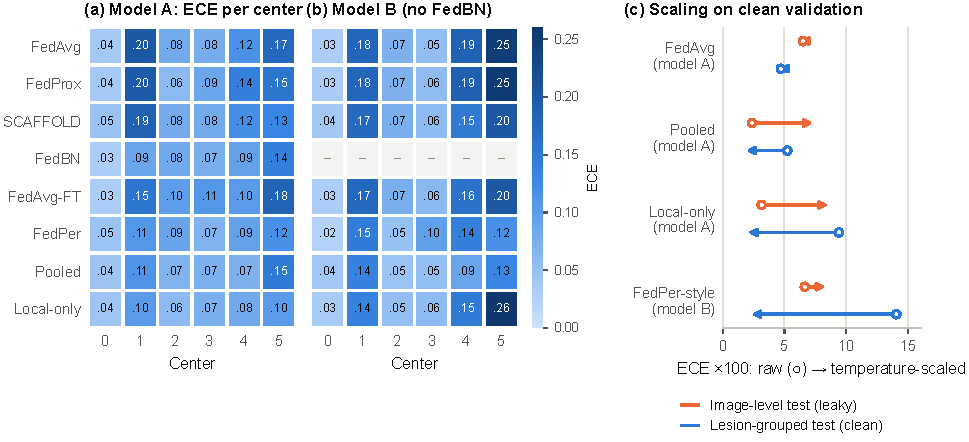
\includegraphics[width=\textwidth]{Fig6_calibration}
  \caption{Calibration. (a, b) Top-label ECE per method and client on lesion-grouped test sets after
  temperature scaling (mean of five seeds; model~B has no FedBN). Values for the small clients 4 and 5 are
  imprecise. (c) ECE ($\times100$) before (open circle) and after temperature scaling fitted on
  lesion-grouped validation data, on image-level (orange) and lesion-grouped (blue) test sets.}
  \label{fig:calibration}
\end{figure*}

\subsection{Federated conformal prediction (RQ1, RQ4)}
\label{sec:res-conformal}

A single global threshold under-covered some clients, as expected for a rule that targets the mixture of
clients, and the pre-specified ShrinkFCP did not fix this (Figure~\ref{fig:conformal};
Table~\ref{tab:conformal}). On the in-federation lesion-grouped FedAvg models (LAC, $\alpha=0.1$), the
global threshold left the worst client at a mean coverage of 0.819 (model~A, client~3) and 0.717 (model~B,
client~4), with worst-client q10 of 0.786 and 0.670; FCP behaved like the global threshold. Client-wise
thresholds gave every client a mean coverage of about 0.90 (worst-client q10 0.794 and 0.795), and the
remaining shortfall in the tail came from the small client~5. ShrinkFCP raised the worst-client q10 of
model~A by 2.5 points over client-wise calibration ($-2.8$ to 3.9) but lowered it by 7.3 points ($-14.0$ to
$-5.4$) for model~B, and for both encoders it violated the mean-coverage guard (lowest client 0.856 and
0.771): RQ4 was not met. The interval for model~A is not centered on the point estimate, because the
bootstrap recomputes q10 from 20 rather than 100 draws per replicate; this is examined below.

On the 18 LOCO models per encoder, the pre-specified test of EB-ShrinkFCP was met for model~A, with a
worst-client q10 of 0.837 against 0.814 for client-wise calibration (gain 2.3 points, 0.8--3.9), set sizes
within 4\% of the reference and every client's mean coverage at least 0.89. The interval supports a gain
above zero, not a gain above 2 points. For model~B the gain was 0.5 points ($-1.7$ to 0.9) and the test was
not met. In all four settings (in-federation and LOCO models, both encoders), EB-ShrinkFCP kept every
client's mean coverage between 0.897 and 0.901, whereas ShrinkFCP dropped the worst client to 0.77--0.86.
On the in-federation models, the post hoc gain of EB-ShrinkFCP over client-wise calibration was 4.8 points
(0.2--6.1) for model~A and 0.1 points for model~B. Per-client set sizes and results for APS scores and for
$\alpha=0.05$ and $0.2$ are given in Supplementary~S5.

Post hoc sensitivity analyses qualify these results (Supplementary~S6). First, q10 estimated from 100 draws
is noisy: for client-wise thresholds on the LOCO models of model~A it ranged from 0.797 to 0.813 across
five independent sets of 100 draws, a spread comparable to the pre-specified gain; with 1,000 draws, the
worst-client q10 was 0.837 for EB-ShrinkFCP and 0.805 for client-wise thresholds (model~A) and 0.805 and
0.797 (model~B). Second, a corrected bootstrap that keeps the resampled copies of a lesion in the same half
gave intervals for the model~A gain over client-wise thresholds of 2.6 to 8.1 points (20 draws per
replicate) and 3.4 to 8.7 (100 draws), and for model~B $-0.3$ to 3.2 and 0.1 to 3.1; these intervals are
not centered on the point estimates, because q10 from resampled clustered data is biased downwards, more
so for the noisier client-wise thresholds. Third, when only one random image per lesion was kept in both
halves, so that calibration and evaluation units are independent lesions, client-wise and EB-ShrinkFCP
thresholds both kept every client's mean coverage at 0.90, and the EB gain in worst-client q10 over
client-wise thresholds was 3.3 points for model~A with an interval that included zero ($-0.4$ to 3.6) and
0.4 points for model~B ($-0.3$ to 1.6); global and FCP thresholds under-covered further (lowest client
0.81 and 0.73). Fourth, when the evaluation half was fixed and only the calibration lesions were redrawn,
EB-ShrinkFCP raised the worst-client q10 over client-wise thresholds by 3.4 points (model~A) and 0.9 points
(model~B), indicating that the gain comes from less variable thresholds rather than from evaluation noise.
Fifth, exact order statistics changed the global and FCP thresholds' q10 by at most 0.003. Finally, the
label-shift-weighted comparator did not repair the per-client shortfall of the global threshold (lowest
client mean coverage 0.85 for model~A and 0.72 for model~B), indicating that the clients differ by more than
their class priors.

On personalized models (FedBN, FedAvg-FT, FedPer and local-only; descriptive), a global threshold still
left some client at a mean coverage of 0.76--0.87, while client-wise thresholds kept every client's mean
coverage between 0.897 and 0.911 and EB-ShrinkFCP between 0.888 and 0.944 (Supplementary~S7).

\begin{figure*}[!t]
  \centering
  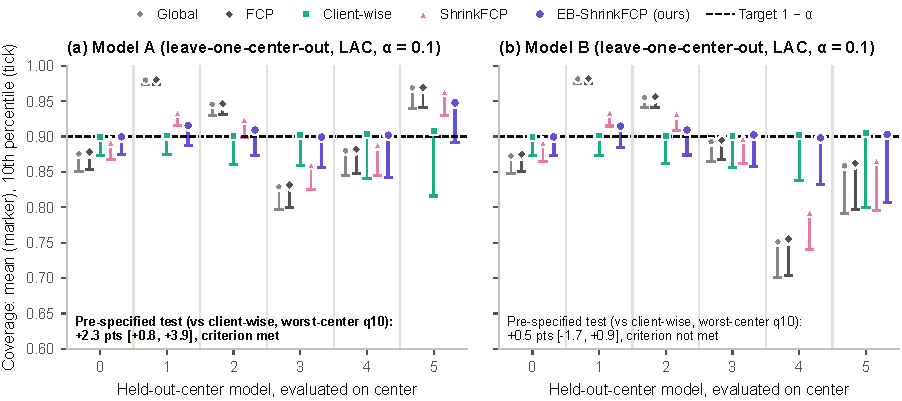
\includegraphics[width=\textwidth]{Fig7_conformal}
  \caption{Federated conformal coverage on LOCO models (LAC, $\alpha=0.1$; 18 models per encoder, 100
  lesion-wise calibration draws each). For each rule and client, the marker is the mean coverage and the
  tick the 10th percentile of coverage over draws (q10), not a confidence interval; dashed line: target
  coverage 0.90. The text gives the pre-specified test of EB-ShrinkFCP against client-wise calibration.}
  \label{fig:conformal}
\end{figure*}

\inputtable{Table4_conformal}

\subsection{Unseen clients and smartphone images (RQ1)}
\label{sec:res-shift}

Accuracy and calibration were worse when a client was unseen in training, and worse still on smartphone
images (Figure~\ref{fig:shift}). On the same held-out test images and seeds, a client held out of training
lost on average 4.6 BA points (model~A) and 5.9 points (model~B) compared with the FedAvg model that
included it; client~0 lost 17.5 and 16.8 points (0.487 to 0.312 and 0.480 to 0.312), and its ECE rose from
0.031 to 0.101 (model~A). For LOCO models, global conformal thresholds left the worst client at a mean
coverage of 0.83 (model~A) and 0.75 (model~B) (Table~\ref{tab:conformal}); because every client, including
the held-out one, was calibrated with its own labelled lesions, client-wise and EB-ShrinkFCP thresholds
reached about 0.90.

On PAD-UFES-20 (closed-set transfer to six shared classes), BA fell from 0.471 on the Fed-ISIC2019
lesion-grouped test set (same six-class restriction) to 0.356 (95\% CI 0.333--0.380) for model~A and from
0.522 to 0.342 (0.320--0.366) for model~B, and ECE rose from 0.058 to 0.190 and from 0.034 to 0.212.
Actinic keratosis, the second most frequent class, was rarely recognized (recall 0.08 and 0.19). Conformal
thresholds transferred from Fed-ISIC2019 covered 0.596 (0.576--0.614) and 0.669 (0.650--0.687) of the
PAD-UFES-20 images instead of 0.90, meeting the pre-specified failure rule; the interval conditions on the
transferred threshold. Recalibrating on half of the PAD-UFES-20 patients restored marginal coverage to
0.900 (10th percentile over draws 0.880 and 0.884), but the prediction sets then contained on average 4.9
(model~A) and 4.3 (model~B) of the six classes, and coverage of actinic keratosis and squamous cell
carcinoma remained between 0.80 and 0.84 (730 and 192 images; about half of each falls in the evaluation half of a draw). The shift combines modality, population, acquisition,
class prevalence and label definitions, so it is not attributable to the imaging device alone.

\begin{figure*}[!t]
  \centering
  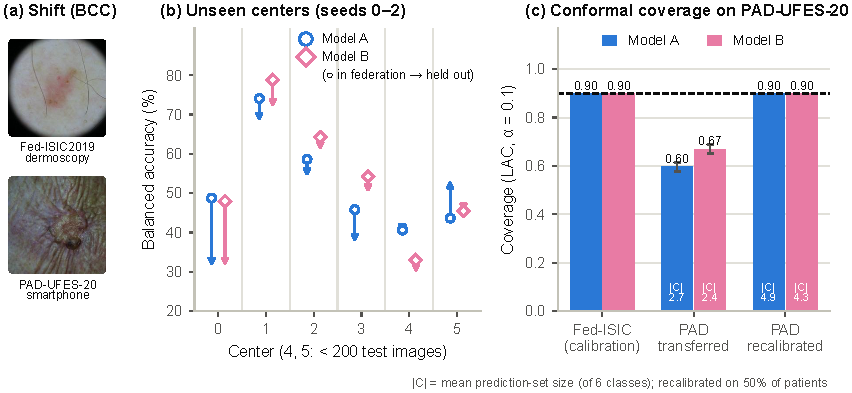
\includegraphics[width=\textwidth]{Fig8_domain_shift}
  \caption{Unseen clients and smartphone images. (a) The same diagnosis (basal cell carcinoma) in a
  Fed-ISIC2019 dermoscopy image and a PAD-UFES-20 smartphone photograph. (b) BA on each client's
  lesion-grouped test set when the client was in the federation (open marker) and when it was held out
  (arrow head); same test images, seeds 0--2. (c) Conformal coverage at $\alpha=0.1$ after the six-class
  restriction: on the Fed-ISIC2019 calibration scores (nominal by construction, shown as reference), on
  PAD-UFES-20 with the transferred threshold (95\% patient-bootstrap CI, conditional on the threshold) and
  after recalibration on 50\% of the patients; $|C|$, mean prediction-set size. Images: ISIC 2019
  (CC-BY-NC 4.0) and PAD-UFES-20 (CC-BY 4.0).}
  \label{fig:shift}
\end{figure*}
